\documentclass{article}
\usepackage[top=1in, bottom=1in, left=1in, right=1in]{geometry}
\usepackage{graphicx}
\usepackage{hhline}
\usepackage{hyperref}
\usepackage{multirow}
\usepackage{url}

\begin{document}
\title{\vspace{-0.5in}SE101---Lab Project}
\author{Rollen D'Souza, Derek Rayside, Patrick Lam}
\date{Fall 2017\\Last Updated \today}
\maketitle

\begin{figure}[ht]
\centering
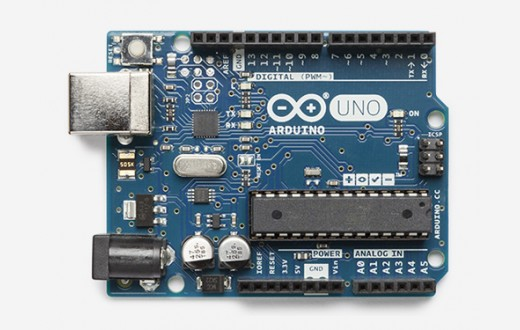
\includegraphics[width=3in]{images/Uno.jpg}
\caption{The Arduino Uno R3~\cite{arduinoUno}}
\label{fig:arduinoUno}
\end{figure}

\section*{Introduction}
This lab gives you the opportunity to follow the full software development cycle and to be creative with a microcontroller board.  You will need to acquire an Arduino Uno R3 (or other Arduino of your choice) and possibly a shield in order to extend functionality.  Only one is required per group.  This lab is flexible.  However, your mark is proportional to both the difficulty of the project you attempt and the performance of your execution.  Keep in mind that you should be able to complete the project with minimal assistance.

\subsection*{Important Dates}
\begin{tabular}{rl}
Proposal Due Date & October 11, 2018 @ 21:00 \quad \emph{Note: This is a logical Tuesday.}\\
Proposal Feedback & October 18, 2018 @ 11:30\\
Prototype Due Date & October 25, 2018 @ 11:30\\
Project Demo Due Date & November 22, 2018 @ 11:30
\end{tabular}

\section*{Requirements}
\begin{itemize}
    \item{Form a group of 2 students and email James Cagalawan your group member Quest/WATIAM IDs}
        \begin{itemize}
            \item James Cagalawan will respond with your project repository on \texttt{git.uwaterloo.ca}.
        \end{itemize}\pagebreak[2]
    \item{Submit a proposal of the project you would like to complete.  The document must:}
        \begin{itemize}
            \item Be a PDF.
            \item Be at most 1 page long.
            \item Be submitted (pushed) to your project group repository as \texttt{proposal.pdf}.
        \end{itemize}\pagebreak[2]
    \item{The proposal must describe the following:}
        \begin{itemize}
            \item Your project.  What will it do?
            \item The major software components of your project (e.g. implement LCD user interface).
            \item Contain a prototype plan as discussed in lecture. This may be a experimental or evolutionary prototype. Which one depends on your choice of project as well as the skills you have available at your disposal.
            \item The hardware you acquire[d] for the project and intend to use.
            \item The challenges you anticipate.  For example: if you are using an LCD screen, you may anticipate the challenge of drawing and moving a complex object.
        \end{itemize}\pagebreak[2]
    \item \emph{If you are unable to formulate a proposal, you must see James Cagalawan in office hours else you forfeit your proposal grade. These are easy marks, don't lose them.}
    \item{You must \emph{develop} and submit the project using \texttt{git.uwaterloo.ca} in the directory provided to your group.  Marks will be deducted for not using source control effectively.  That is, we expect to see at least two non-trivial commits.  Trivial commits are those that consist of only changes to whitespace.}
\end{itemize}

\section*{Marking Scheme}
\begin{center}
\begin{tabular}[c]{cr|c}
& \textbf{Criterion} & \textbf{Mark Contribution} \\ \hline

& Project Proposal & 5 \\ \hline

& Initial Prototype & 10 \\ \hline

\multirow{3}{*}{Execution}
    & Low Difficulty &  10 \\
    & Average Difficulty & 10 \\
    & Above Average Difficulty & 10 \\ \hline

\multirow{5}{*}{Style}
    & Naming &  1 \\
    & Whitespace Usage & 1\\
    & Easy to Modify & 1\\
    & Use of Control Flow and Types & 1\\
    & Use of Source Control & 1\\ \hhline{==|=}

& Total & 50 \\ \hhline{==|=}
& Bonus &
\end{tabular}
\end{center}

\section*{Suggested Resources}
\begin{itemize}
    \item Although you can acquire the \href{https://store.arduino.cc/usa/arduino-uno-rev3}{official} Arduino Uno R3, you might find cheaper alternatives made by SainSmart or Elegoo.  We have tried the \href{https://www.amazon.ca/gp/product/B01EWOE0UU/}{Elegoo brand} and have found no apparent differences yet paid \$14 each.
    \item There are a variety of shields out there.  Ensure that, if you purchase a shield, it \emph{comes with the header pins attached}.  If it doesn't, you'll have to solder them on yourself.
    \item There are a number of LCD character display shields available, with buttons, such as \href{https://www.amazon.ca/gp/product/B01C9V7U8W/}{this} or \href{http://www.robotshop.com/ca/en/lcd12864-lcd-shield-arduino-compatible.html}{this}~.  Keep in mind every shield is different, so keep a look out for what features are available, and what aren't!
    \item The RigidWare store --- operated by EngSoc --- has a decent amount of hardware available for you to purchase, including Arduinos.
    \item There are options for if your project really doesn't work out; talk to James if disaster strikes.
\end{itemize}

\section*{Suggested Projects}
\begin{itemize}
    \item Mimic a clock app on the phone. e.g. keep track of time, implement an alarm clock, implement a stop watch, support UTC.
    \item Make a small game on a computer and turn your Arduino into a controller.
    \item Make a game on the Arduino with a LCD shield (make sure it isn't just a character display!)
\end{itemize}

\section*{Submission}
You must submit your project into the provided \texttt{git.uwaterloo.ca} repository.  You are graded on your use of \texttt{git}.  We expect to see at least two non-trivial commits.  Trivial commits are those that consist of only changes to whitespace.  Email James or Xiao if you can't commit to that address.

\section*{Tips}
\begin{itemize}
    \item The moment you have a working program, commit it!  If things go wrong, you can always go back.
    \item Expect to stumble upon unexpected hurdles.  Always give yourself an ample amount of time to finish the project!
\end{itemize}

\begin{flushleft}
\begin{thebibliography}{1}
\bibitem{arduinoUno}
    Arduino.
    (2017).
    \emph{Arduino Uno Rev3 - Boards \& Modules - Arduino}.
    \url{https://store.arduino.cc/usa/arduino-uno-rev3}
\end{thebibliography}
\end{flushleft}

\end{document}
